\documentclass[tikz,border=10pt]{standalone}
\usetikzlibrary{arrows.meta,calc,positioning}

\begin{document}
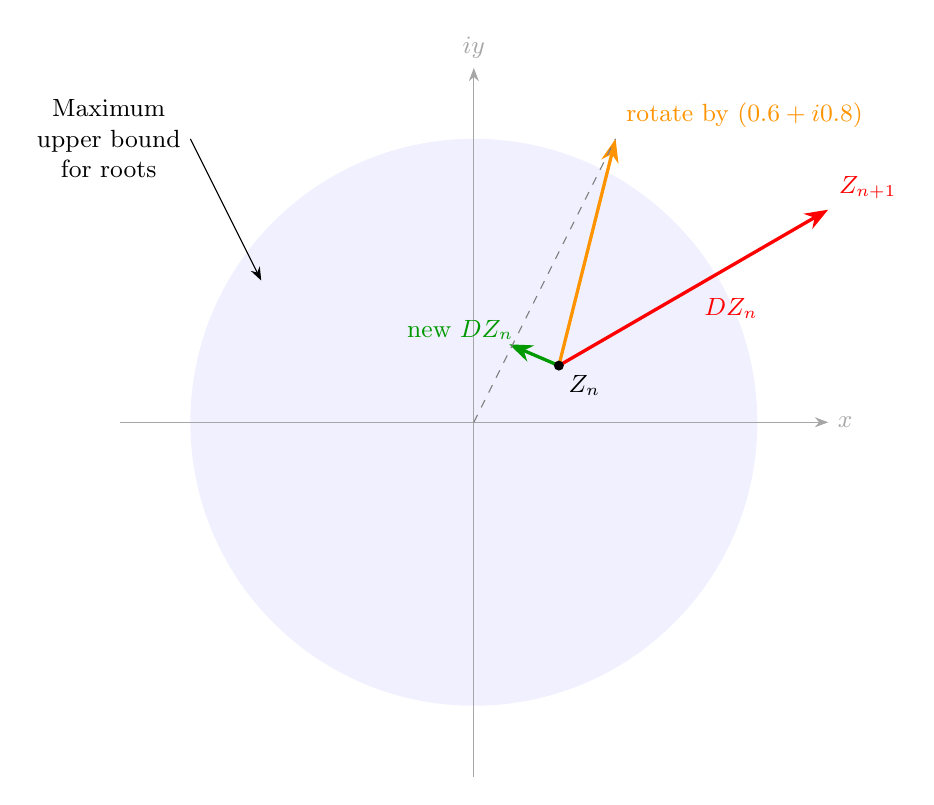
\begin{tikzpicture}[>=Stealth,             % arrow style
                    scale=0.9,
                    every node/.style={font=\small}]

% ---------------------------------------------------------------
% Key points
\coordinate (O)   at (0,0);          % circle centre
\coordinate (Zn)  at (1.2,0.8);      % Z_n
\coordinate (Znp) at (5,3);          % Z_{n+1}  (red tip)
\coordinate (Yend)at (2,4);      % yellow tip  (rotated DZn)

% Foot of perpendicular from Zn onto line O--Yend (computed once)
\coordinate (Gend) at (0.5,1.1); % new DZ_n (green tip)

% ---------------------------------------------------------------
% Disks (flat fill, no 3‑D effect)
\fill[blue!20,opacity=0.3] (O) circle (4);  % outer bound


% Axes
\draw[gray!70,->] (-5,0) -- (5,0) node[right] {$x$};
\draw[gray!70,->] (0,-5) -- (0,5) node[above] {$iy$};

% Arrows
\draw[very thick,red,->]   (Zn) -- (Znp)
      node[pos=0.5,below right] {$DZ_{n}$}
      node[above right] {$Z_{n+1}$};

\draw[very thick,orange!85!yellow,->] (Zn) -- (Yend)
      node[pos=1.0,above right] {rotate by $(0.6+i0.8)$};

\draw[very thick,green!60!black,->]   (Zn) -- (Gend)
      node[pos=0.7,above left] {new $DZ_{n}$};

% Helper dashed line showing perpendicular relation
\draw[dashed,gray] (O) -- (Yend);

% Label for maximum bound
\draw[->] (-4,4) -- (-3,2)
      node[pos=0,left,align=center] {Maximum\\upper bound\\for roots};

% Mark Z_n
\fill (Zn) circle (2pt) node[below right] {$Z_n$};

\end{tikzpicture}
\end{document}
